\section{Smote and under-sampling technique}

SMOTE (Synthetic Minority Over-sampling Technique) is an oversampling method used to generate synthetic samples for the minority class. Despite experimenting with SMOTE, random over-sampling, and under-sampling techniques, the results on the validation data were poor.


\begin{figure}[h]
    \centering
    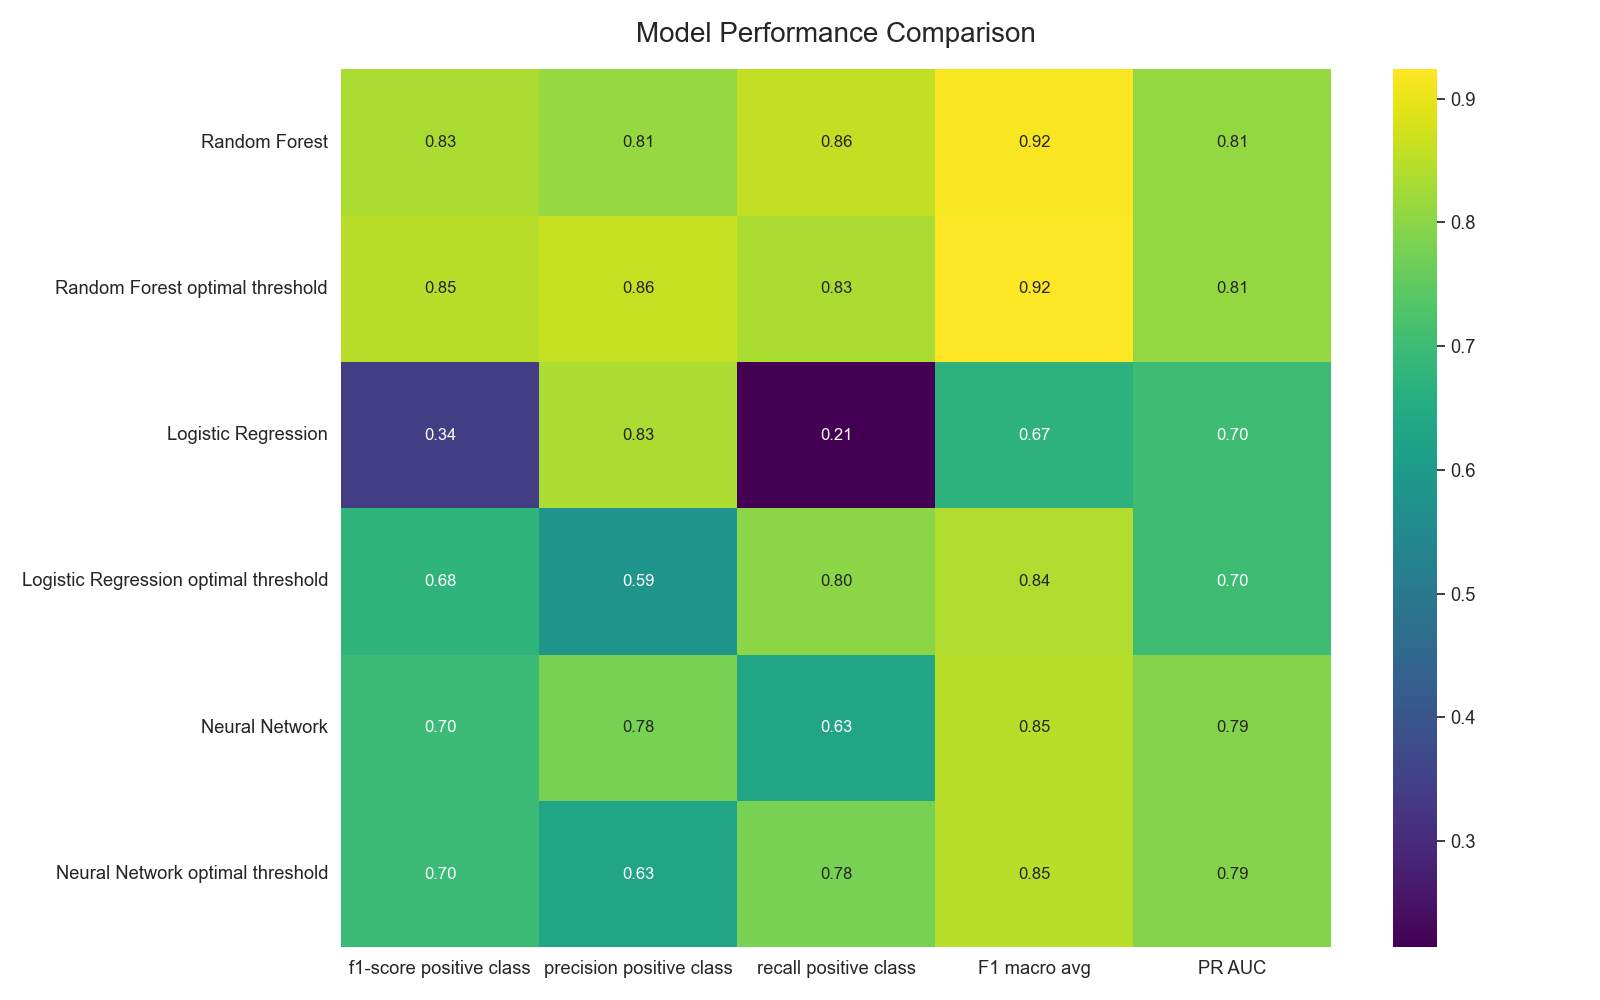
\includegraphics[width=0.80\linewidth]{Smote (0.05-ratio).png}
    \caption{Smote (0.05-ratio)}
    \label{fig:Smote (0.05-ratio)}
\end{figure}

\begin{figure}[h]
    \centering
    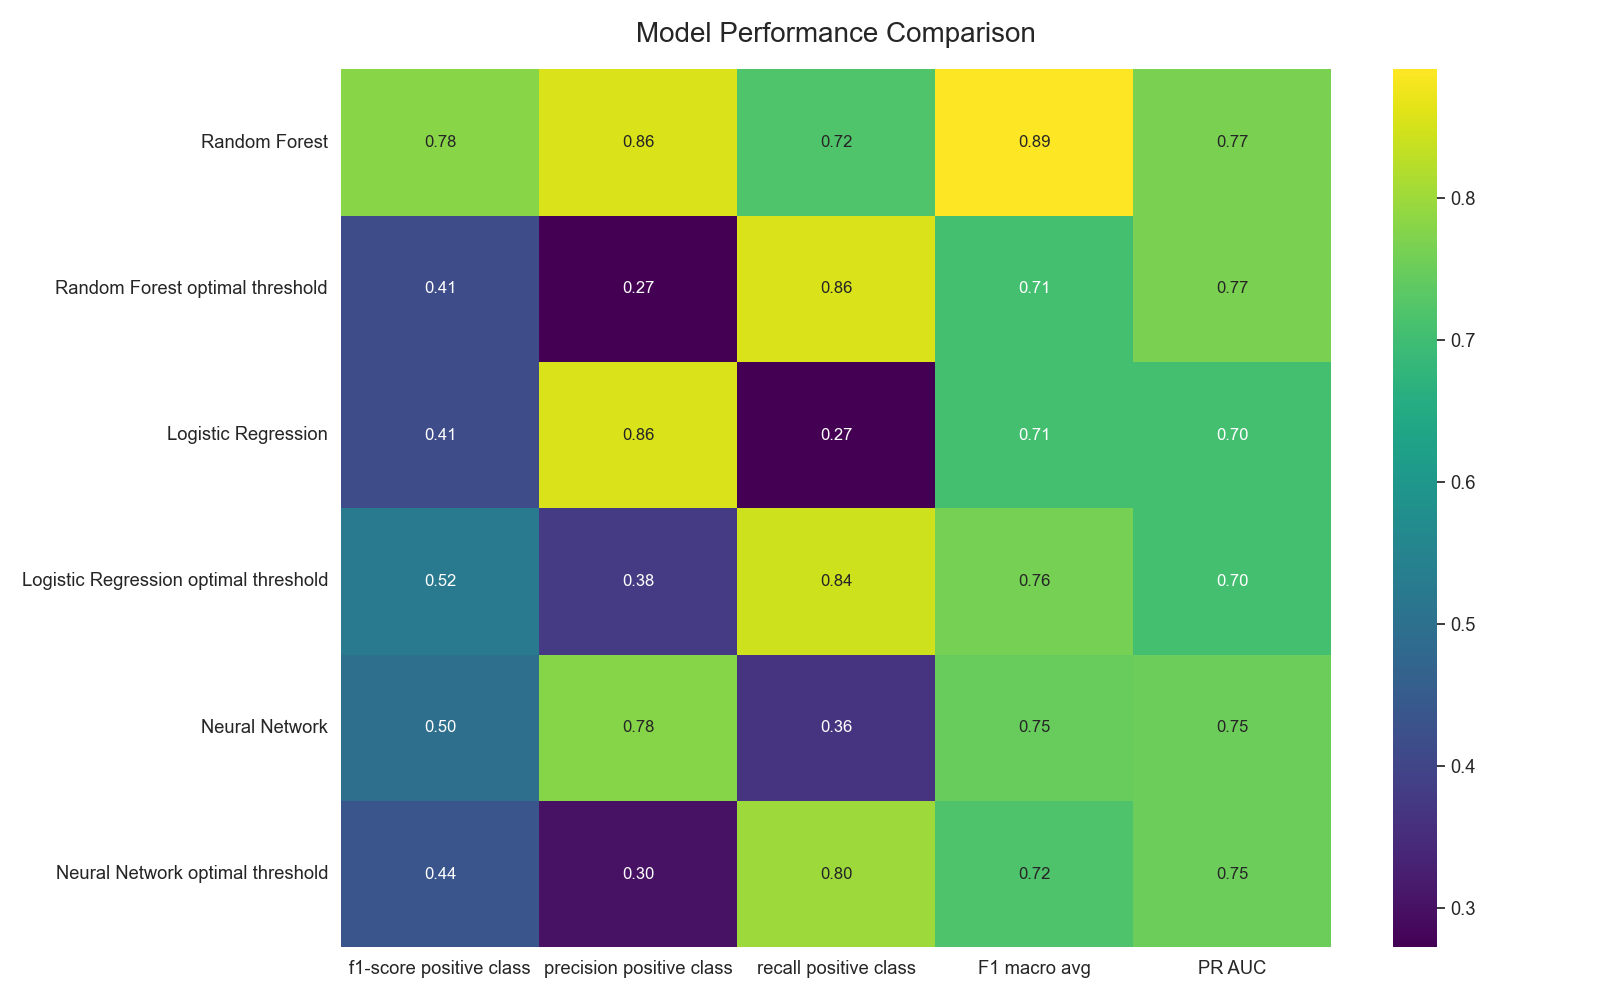
\includegraphics[width=0.80\linewidth]{RandomUnderSampler (0.05-ratio) results.png}
    \caption{Random-Under-Sampler (0.05-ratio) result}
    \label{fig:enter-label}
\end{figure}